\chapter{Modèle proposé et architecture d'Ariel Logminer}
\label{chap:architecture}

\section{Introduction}

L'état de l'art a montré que l'analyse de journaux hétérogènes ne peut pas être réduite
au choix d'un seul algorithme de détection. Avant qu'un modèle puisse produire un résultat,
les données doivent être acquises, reconnues, transformées et orientées vers un traitement
compatible. Après la détection, les sorties doivent encore être contextualisées, conservées,
corrélées et présentées à l'analyste. Ces fonctions appartiennent à des domaines différents,
mais elles doivent coopérer dans une même chaîne.

Ariel \logminer{} est conçu pour répondre à ce problème d'intégration. Son architecture
sépare les principales responsabilités du traitement afin qu'un composant puisse évoluer
sans imposer une réécriture complète des autres. Cette séparation facilite également
l'audit : lorsqu'une anomalie candidate paraît incohérente, il doit être possible de
déterminer si le problème provient de la lecture de la source, du parsing, de la
normalisation, du routage, du modèle ou de la corrélation.

Le système est qualifié de multi-agent parce que plusieurs composants spécialisés disposent
de capacités, d'un état et d'un mécanisme de communication. Il est distribué dans le sens
où certaines tâches peuvent être confiées à des workers distincts et transportées au moyen
de Redis Streams. Cette distribution reste cependant une distribution logicielle et de
laboratoire. Elle n'implique ni haute disponibilité industrielle ni fonctionnement
géographiquement distribué.

Le présent chapitre expose le modèle architectural final du prototype. Il présente d'abord
les exigences et principes de conception, puis décrit les composants, le cycle de vie des
données, les contrats de communication, le routage, la mémoire, la corrélation et la
gouvernance des modèles. Les détails de programmation sont volontairement reportés au
chapitre suivant afin de maintenir une distinction claire entre \textit{conception} et
\textit{implémentation}.

\section{Exigences de conception}

\subsection{Exigences fonctionnelles}

La conception part d'une chaîne fonctionnelle complète. Pour qu'une source puisse être
exploitée, le système doit être capable de la recevoir, d'en déterminer la nature,
d'extraire les informations utiles et de transmettre une représentation exploitable aux
composants suivants.

Les principales exigences fonctionnelles sont synthétisées dans le
tableau~\ref{tab:exigences-fonctionnelles}.

\begin{table}[H]
\centering
\caption{Exigences fonctionnelles principales d'Ariel \logminer{}}
\label{tab:exigences-fonctionnelles}
\small
\begin{tabularx}{\textwidth}{p{1.2cm}p{4.0cm}X}
\toprule
\textbf{ID} & \textbf{Fonction} & \textbf{Exigence} \\
\midrule

F1 & Acquisition &
Accepter plusieurs catégories de fichiers, journaux ou exports utilisés dans le périmètre
du prototype. \\

F2 & Parsing &
Extraire les champs pertinents d'une source lorsque son format est reconnu et signaler
explicitement les cas non pris en charge. \\

F3 & Normalisation &
Transformer les informations disponibles vers un noyau commun exploitable par les
composants transversaux. \\

F4 & Routage &
Identifier une famille probable de données et choisir un traitement compatible. \\

F5 & Détection &
Appliquer un modèle supervisé, non supervisé ou statistique selon la nature de la source
et le protocole prévu. \\

F6 & Corrélation &
Rapprocher plusieurs anomalies candidates à partir d'indices temporels ou contextuels. \\

F7 & Mémoire et audit &
Conserver les informations nécessaires à la traçabilité des exécutions, décisions et
erreurs. \\

F8 & Visualisation &
Présenter les résultats sous une forme permettant leur consultation, leur filtrage et leur
inspection par l'analyste. \\

F9 & Mise à jour contrôlée &
Comparer un modèle candidat au modèle courant avant toute décision de promotion. \\

\bottomrule
\end{tabularx}
\end{table}

Ces fonctions ne sont pas toutes évaluées de la même manière. Une opération de parsing
peut être vérifiée par le nombre d'entrées effectivement transformées. La qualité d'un
classifieur nécessite des métriques de prédiction. Le bus de messages demande des mesures
d'acquittement et de reprise. Le tableau de bord peut être vérifié fonctionnellement sans
que cela constitue pour autant une étude d'utilisabilité.

Cette distinction entre fonction et preuve associée est intégrée dès la conception.

\subsection{Exigences non fonctionnelles}

Cinq exigences non fonctionnelles structurent l'architecture.

La première est la \textbf{modularité}. Chaque composant doit assumer une responsabilité
principale identifiable. Le routeur ne doit pas effectuer lui-même l'entraînement d'un
modèle ; le corrélateur ne doit pas remplacer le normaliseur ; le dashboard ne doit pas
constituer l'unique emplacement où une décision est enregistrée.

La deuxième est l'\textbf{auditabilité}. Les traitements importants doivent laisser des
traces permettant de comprendre ce qui s'est produit. Dans un contexte de cybersécurité,
un résultat difficile à expliquer possède une valeur limitée, même lorsqu'il est obtenu
avec un modèle performant.

La troisième est la \textbf{reproductibilité}. Les données, paramètres, versions de
modèles et artefacts expérimentaux doivent pouvoir être associés aux résultats qui en
découlent.

La quatrième est la \textbf{dégradation contrôlée}. Une source inconnue ou mal formée ne
doit pas être silencieusement considérée comme correctement traitée. Lorsque le système
ne sait pas appliquer le chemin nominal, il doit pouvoir utiliser une route de repli,
enregistrer l'erreur ou conserver les éléments disponibles.

La cinquième exigence est la \textbf{sobriété opérationnelle}. Le prototype doit rester
exécutable dans un environnement local raisonnable. L'architecture autorise une extension
vers une distribution plus large, mais ne dépend pas d'un cluster industriel pour assurer
ses fonctions essentielles.

\section{Principes architecturaux}

\subsection{Séparation des responsabilités}

Le premier principe consiste à éviter qu'un seul module prenne en charge toute la chaîne.
Cette décomposition répond à deux besoins.

Le premier est technique. Les sources sont hétérogènes et les algorithmes ne partagent pas
nécessairement les mêmes entrées. Une étape de normalisation doit donc être distincte du
modèle qui consomme les données.

Le second est méthodologique. Lorsque chaque étape est identifiable, il devient possible
d'évaluer séparément le comportement du parser, du routeur ou du détecteur. Une erreur du
routeur ne doit pas être interprétée comme une erreur intrinsèque du modèle.

\subsection{Séparation entre contrat métier et transport}

Le deuxième principe concerne la communication entre composants.

Le message utilisé par les agents décrit une intention métier : qui envoie, qui reçoit,
quel type de message est transporté et quelle charge utile doit être traitée.

Le bus possède, de son côté, ses propres besoins : identifiant de stream, groupe de
consommateurs, statut pending, acquittement ou reprise.

Ces deux niveaux ne doivent pas être confondus. Un identifiant généré par Redis pour
acquitter un message n'est pas automatiquement l'identifiant métier de l'événement de
sécurité analysé.

\subsection{Autonomie encadrée}

Le troisième principe est celui d'une autonomie limitée et vérifiable.

Le système peut réaliser automatiquement plusieurs actions : découvrir une source,
calculer des indices de routage, sélectionner un traitement, exécuter un modèle, produire
une anomalie candidate ou publier une tâche.

Il ne doit cependant pas transformer automatiquement tout score inhabituel en incident
confirmé, ni remplacer un modèle courant sans comparaison préalable. Les décisions à
forte portée restent encadrées par des règles explicites ou par une validation humaine.

\subsection{Conservation des résultats négatifs}

Le quatrième principe concerne l'évaluation. L'architecture n'est pas conçue uniquement
pour confirmer les hypothèses initiales. Une voie de normalisation qui échoue, un modèle
qui ne généralise pas ou un système à agents plus lent qu'une version monolithique doivent
rester visibles.

Ce principe influence l'audit et la persistance : les erreurs et rejets ne sont pas
considérés comme des informations inutiles à supprimer.

\section{Architecture générale}

La figure~\ref{fig:architecture-finale} représente l'architecture logique finale du
prototype. Elle ne contient volontairement aucune information de version ou d'historique
de développement.

\begin{figure}[H]
\centering

\resizebox{0.98\textwidth}{!}{%
\begin{tikzpicture}[
node distance=0.85cm and 0.95cm,
component/.style={
    draw,
    rounded corners=2pt,
    align=center,
    minimum width=2.45cm,
    minimum height=0.9cm,
    font=\small
},
store/.style={
    draw,
    cylinder,
    shape border rotate=90,
    aspect=0.25,
    align=center,
    minimum width=2.5cm,
    minimum height=0.9cm,
    font=\small
},
arrow/.style={-{Latex[length=2.2mm]}, thick},
feedback/.style={-{Latex[length=2.2mm]}, dashed, thick}
]

\node[component] (sources) {Sources\\de journaux};
\node[component, right=of sources] (collect) {Collecte\\et lecture};
\node[component, right=of collect] (parse) {Parsing};
\node[component, right=of parse] (norm) {Normalisation};
\node[component, right=of norm] (route) {Routage};

\node[component, below=1.25cm of route] (detect) {Détection};
\node[component, left=of detect] (corr) {Corrélation};
\node[component, left=of corr] (dash) {Dashboard\\et analyste};

\node[store, below=1.20cm of norm] (audit) {Audit\\et mémoire};
\node[component, right=of detect] (update) {Mise à jour\\contrôlée};

\node[component, below=1.20cm of detect] (bus) {Bus de tâches\\local / Redis / MQTT};

\draw[arrow] (sources) -- (collect);
\draw[arrow] (collect) -- (parse);
\draw[arrow] (parse) -- (norm);
\draw[arrow] (norm) -- (route);
\draw[arrow] (route) -- (detect);
\draw[arrow] (detect) -- (corr);
\draw[arrow] (corr) -- (dash);

\draw[feedback] (collect) -- (audit);
\draw[feedback] (parse) -- (audit);
\draw[feedback] (route) -- (audit);
\draw[feedback] (detect) -- (audit);
\draw[feedback] (corr) -- (audit);
\draw[feedback] (dash) -- (audit);

\draw[feedback] (audit) -- (update);
\draw[feedback] (update) -- (route);

\draw[arrow] (bus) -- (detect);
\draw[feedback] (bus) -- (audit);

\end{tikzpicture}
}

\caption{Architecture logique finale d'Ariel \logminer{}.}
\label{fig:architecture-finale}
\end{figure}

\begin{center}
\footnotesize Source : auteur.
\end{center}

Le flux principal se lit de gauche à droite. Une source est d'abord acquise ou ouverte.
Le parser extrait les informations qu'il reconnaît. Le normaliseur tente ensuite de
construire une représentation commune. Le routeur détermine la famille la plus plausible
et sélectionne le traitement correspondant. Le détecteur produit un score, une classe ou
une décision intermédiaire selon le type de modèle. Les anomalies candidates peuvent alors
être transmises au corrélateur puis au tableau de bord.

L'audit et la mémoire ne constituent pas une étape terminale unique. Ils sont représentés
comme une fonction transversale parce que plusieurs composants peuvent y enregistrer des
informations. Une erreur de parsing, une décision de routage, un résultat de modèle ou un
feedback analyste possèdent tous un intérêt pour la traçabilité.

Le bus de tâches est également transversal. Le pipeline peut être exécuté localement sans
que toutes les opérations passent obligatoirement par Redis. Redis Streams intervient
lorsque les tâches doivent être distribuées entre workers. MQTT représente une autre voie
de communication prévue par le contrat logiciel. Ces mécanismes de transport ne modifient
pas la signification métier d'un message.

\section{Organisation en plans fonctionnels}

Pour faciliter l'analyse, l'architecture peut être divisée en quatre plans.

\subsection{Plan de données}

Le plan de données regroupe les transformations qui modifient directement la représentation
d'une source :

\begin{center}
\textit{source}
$\longrightarrow$
\textit{lecture}
$\longrightarrow$
\textit{parsing}
$\longrightarrow$
\textit{normalisation}
$\longrightarrow$
\textit{détection}.
\end{center}

Chaque étape reçoit une représentation et produit une représentation plus adaptée au
traitement suivant.

\subsection{Plan d'orchestration}

Le plan d'orchestration décide quel composant doit intervenir et comment une tâche peut
être transportée.

Il contient notamment :

\begin{itemize}
    \item le routage par famille ;
    \item le choix du modèle ou du handler ;
    \item l'affectation de tâches à des agents ;
    \item les heartbeats ;
    \item les consumer groups Redis ;
    \item les mécanismes d'acquittement et de reprise prévus.
\end{itemize}

Ce plan correspond principalement au sens donné aux termes \textit{autonome} et
\textit{distribué} dans le mémoire.

\subsection{Plan de persistance et d'audit}

Le plan de persistance conserve les éléments nécessaires pour expliquer ou reproduire une
exécution.

Il peut comprendre :

\begin{itemize}
    \item fichiers de résultats ;
    \item historiques d'exécution ;
    \item décisions de routage ;
    \item scores ;
    \item erreurs ;
    \item feedback analyste ;
    \item versions de modèles ;
    \item hashes d'intégrité ;
    \item décisions de promotion ou de rejet.
\end{itemize}

Ce plan est particulièrement important pour distinguer une simple application qui affiche
un résultat d'un prototype scientifique dans lequel les résultats doivent rester
rattachables à des preuves.

\subsection{Plan de contrôle humain}

Le quatrième plan concerne l'analyste.

Le système peut automatiser la préparation et la priorisation des signaux, mais il ne
supprime pas le besoin d'une interprétation humaine. Le dashboard expose les informations
nécessaires à cette inspection et permet, lorsqu'une fonction correspondante est
disponible, d'enregistrer une validation, un rejet ou un reclassement.

Cette décision peut ensuite être conservée dans la mémoire et l'audit. Elle ne modifie pas
directement un modèle en production.

\section{Agents fonctionnels}

Dans ce mémoire, un agent est un composant logiciel spécialisé. Le terme ne désigne pas
une entité cognitive générale.

Les responsabilités principales sont résumées dans le
tableau~\ref{tab:agents-architecture}.

\begin{table}[H]
\centering
\caption{Responsabilités des agents et composants fonctionnels}
\label{tab:agents-architecture}
\small
\begin{tabularx}{\textwidth}{p{3.1cm}X X}
\toprule
\textbf{Composant} &
\textbf{Responsabilité principale} &
\textbf{Sortie attendue} \\
\midrule

Collecteur &
Découvrir ou charger une source disponible dans le périmètre du prototype. &
Objet, fichier ou unité de travail associée à une provenance. \\

Parseur &
Reconnaître la structure d'une entrée et extraire les champs disponibles. &
Événement parsé ou erreur/fallback explicite. \\

Normaliseur &
Projeter les informations disponibles vers un noyau commun. &
Événement normalisé lorsque la voie le permet. \\

Routeur &
Estimer la famille de la source et sélectionner un modèle ou handler compatible. &
Famille, traitement choisi, scores heuristiques et justification. \\

Détecteur &
Appliquer le traitement statistique ou ML associé à la famille. &
Classe, score ou anomalie candidate selon le modèle. \\

Corrélateur &
Regrouper des anomalies candidates qui présentent des relations compatibles. &
Incident candidat ou groupe corrélé. \\

Audit &
Enregistrer les informations nécessaires à la traçabilité. &
Historique inspectable des opérations et décisions. \\

Mémoire &
Conserver certains états et retours utiles aux traitements ultérieurs. &
Informations persistantes accessibles aux mécanismes autorisés. \\

Dashboard &
Présenter les événements et permettre leur inspection. &
Vue analyste, filtres et décisions lorsque disponibles. \\

Superviseur / workers &
Distribuer, sélectionner et suivre certaines tâches. &
État d'exécution, heartbeat, acquittement ou erreur. \\

\bottomrule
\end{tabularx}
\end{table}

La séparation n'interdit pas qu'un même processus exécute plusieurs responsabilités dans
un scénario local. Elle définit plutôt des frontières logiques. Ces frontières deviennent
particulièrement utiles lorsqu'une partie du pipeline est exécutée par plusieurs workers.

\subsection{Architecture multi-agents réellement utilisée}

Le chemin multi-agents évalué s'appuie sur \texttt{MultiTaskIntelligentAgent} et
\texttt{ContractNetCoordinator}. Le premier regroupe plusieurs capacités et handlers, observe son
état local, calcule une offre ou un refus et conserve un feedback lorsque la mémoire est
activée. Le second enregistre les agents, diffuse les appels à propositions, compare les
utilités reçues, attribue la tâche, rejette les autres offres et écrit la trace du cycle.
Le coordinateur ne calcule donc pas l'utilité à la place des agents.

Les variantes de transport et de persistance sont séparées du contrat métier :
\texttt{LocalMessageBus} et \texttt{RedisMessageBus} transportent les messages ;
\texttt{RedisContractNetCoordinator} et \texttt{RedisContractNetTransport} réalisent la négociation
inter-processus ; \texttt{SQLiteIdempotencyStore} et \texttt{RedisIdempotencyStore} empêchent une
réexécution contrôlée lorsqu'une clé a déjà produit un résultat. Cette organisation permet
de tester le même protocole en local, sur plusieurs processus et dans deux machines
virtuelles.

Le cycle de négociation est :

\begin{center}
\textit{CFP} $\rightarrow$ \textit{PROPOSE/REFUSE}
$\rightarrow$ \textit{AWARD/REJECT} $\rightarrow$ \textit{ACCEPT}
$\rightarrow$ \textit{RESULT/FAIL} $\rightarrow$ \textit{FEEDBACK}.
\end{center}

La politique initiale fixe l'utilité expérimentale à
\[
U=0{,}30C+0{,}20H+0{,}20M+0{,}15A+0{,}10L+0{,}05T,
\]
avec des composantes bornées entre 0 et 1. La fiabilité historique est calculée par
$H_i=(s_i+1)/(s_i+f_i+2)$. Les poids sont configurables et fixés avant les campagnes ;
ils ne sont pas appris et ne sont pas présentés comme optimaux.

Le superviseur historique reste disponible comme architecture centralisée de comparaison.
Il ne doit pas être confondu avec le chemin autonome évalué, dans lequel les agents
proposent ou refusent localement avant l'attribution.

\begin{figure}[H]
\centering
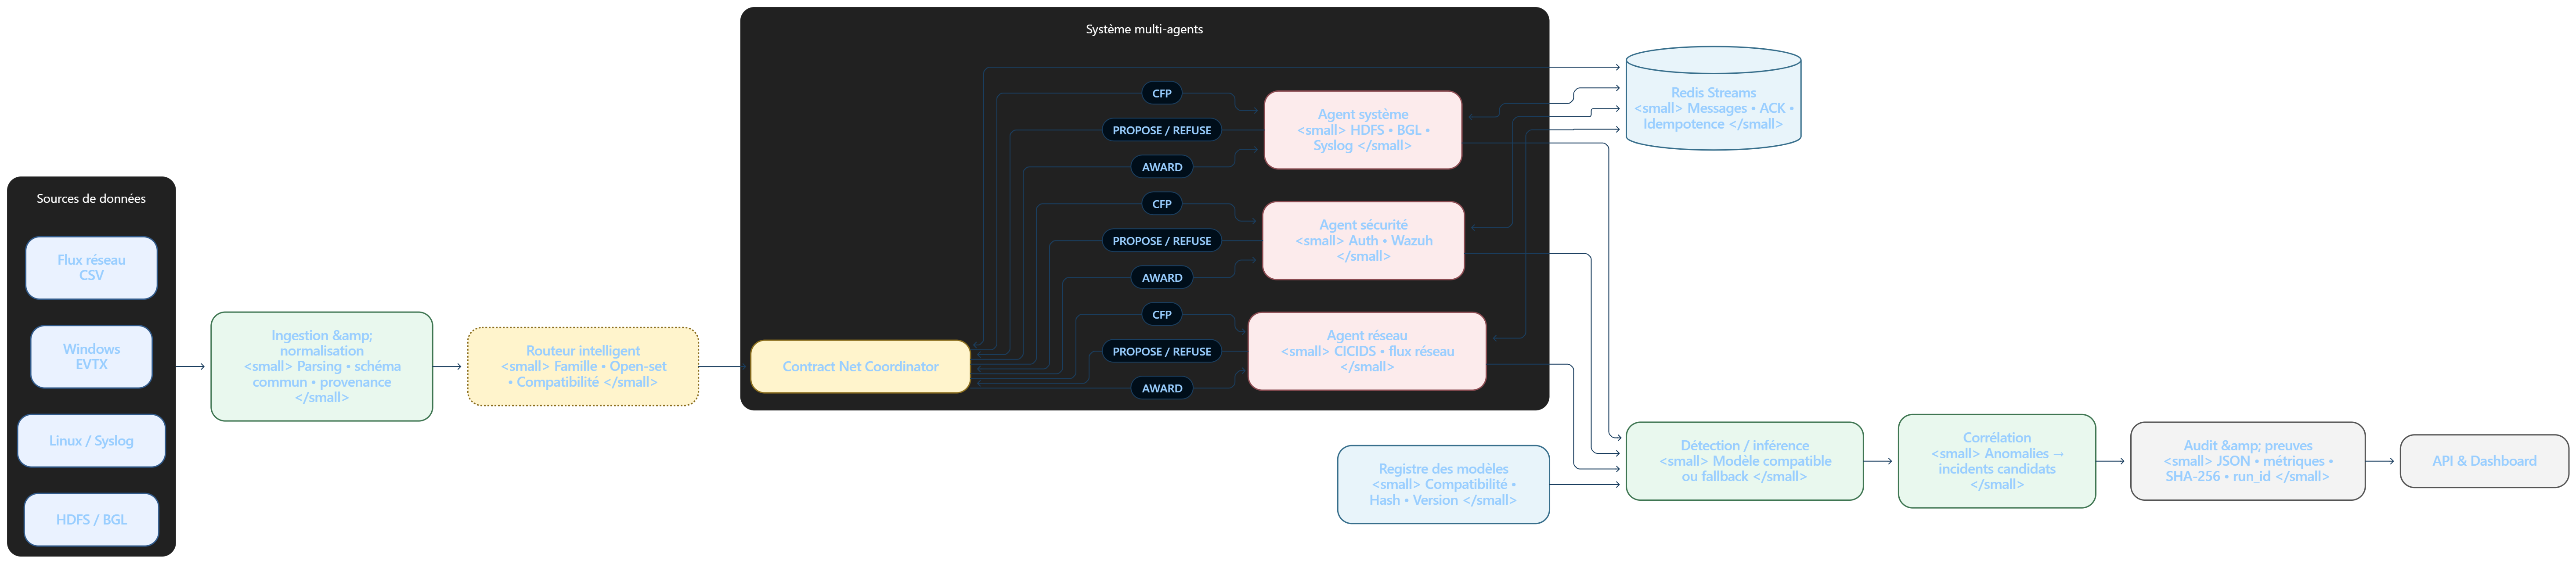
\includegraphics[width=\textwidth]{figures/final/fig_architecture_multi_agent_global.png}
\caption{Architecture multi-agents effectivement évaluée. Le diagramme relie les sources,
la normalisation, le routage, le Contract Net, le transport Redis et les artefacts de preuve ;
il ne constitue pas une spécification de déploiement industriel.}
\label{fig:architecture-multi-agent-finale}
\end{figure}

\begin{figure}[H]
\centering
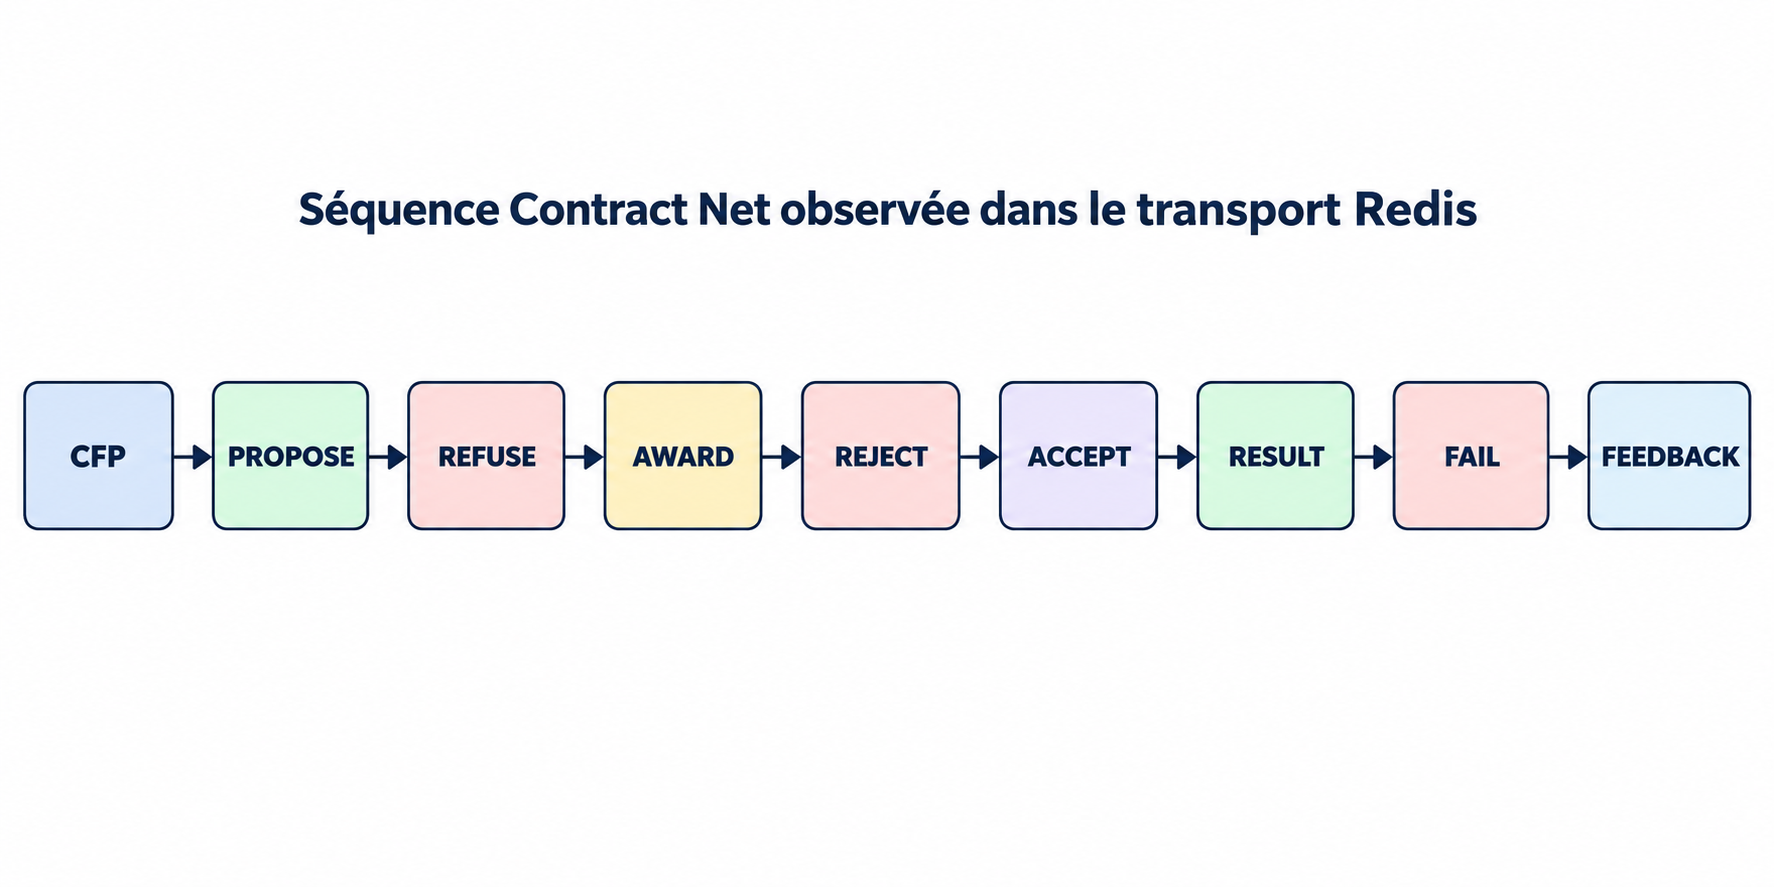
\includegraphics[width=\textwidth]{figures/final/fig_contract_net_sequence.png}
\caption{Séquence Contract Net observée dans les campagnes locales et Redis. Les branches
\textit{REFUSE} et \textit{FAIL} sont conservées pour rendre visibles les reprises contrôlées.}
\label{fig:contract-net-sequence-finale}
\end{figure}

\section{Cycle de vie d'une donnée}

\subsection{Niveau 1 : source brute}

Le premier niveau correspond à l'objet reçu du système ou du fichier d'origine.

Il peut s'agir d'une ligne textuelle, d'un enregistrement tabulaire, d'un événement
Windows, d'un export de plateforme de sécurité ou d'un objet déjà structuré.

À ce stade, aucune hypothèse forte n'est faite sur sa compatibilité avec les modèles.

\subsection{Niveau 2 : événement parsé}

Le parser tente d'extraire les informations significatives.

L'événement parsé reste proche de la structure de sa source. Par exemple, un export
tabulaire peut conserver ses colonnes spécifiques tandis qu'un message système peut être
décomposé en timestamp, hôte, composant et message lorsque ces informations sont
disponibles.

Cette étape doit également pouvoir produire un constat d'échec. Une entrée non reconnue
ne doit pas être considérée comme correctement parsée.

\subsection{Niveau 3 : événement normalisé}

Le niveau normalisé introduit un noyau commun.

L'objectif est de permettre à plusieurs composants transversaux d'accéder à des concepts
similaires sans connaître tous les formats d'origine.

Le noyau peut notamment contenir des informations telles que :

\begin{itemize}
    \item horodatage ;
    \item source ;
    \item hôte ;
    \item famille ;
    \item catégorie ;
    \item sévérité ;
    \item message ;
    \item données spécifiques nécessaires à la suite du traitement.
\end{itemize}

Il serait toutefois incorrect d'affirmer que toutes les sources traversent toujours cette
étape sans perte. Le modèle architectural prévoit une normalisation commune, tandis que
sa couverture réelle dépend des adaptateurs effectivement implémentés. Cette propriété est
mesurée dans le chapitre expérimental.

\subsection{Niveau 4 : sortie de détection}

Après sélection du traitement, le système produit une sortie qui dépend de la nature du
modèle.

Dans un scénario supervisé, la sortie peut être une classe ou un score de classification.
Dans un scénario non supervisé, elle correspond plutôt à un score d'anomalie ou à une
décision dérivée d'un seuil.

Le système conserve la différence sémantique entre ces deux catégories. Un score
d'anomalie n'est pas transformé automatiquement en attaque confirmée.

\subsection{Niveau 5 : anomalie candidate}

Lorsqu'une sortie satisfait le critère de sélection du détecteur, elle devient une anomalie
candidate.

Ce changement de niveau signifie simplement que l'observation mérite davantage
d'attention. Il ne constitue pas une validation de sécurité.

\subsection{Niveau 6 : incident candidat}

Le corrélateur peut rapprocher plusieurs anomalies candidates lorsque des relations
temporelles ou contextuelles sont observées.

Le résultat est appelé \textit{incident candidat} ou groupe corrélé. Là encore, ce terme
ne remplace pas la confirmation humaine d'un incident réel.

\subsection{Niveau 7 : décision analyste}

Le dernier niveau correspond à l'interprétation disponible après inspection.

L'analyste peut, selon les fonctions de l'interface, conserver un statut, confirmer
l'intérêt d'un signal, le rejeter ou le reclasser.

Cette progression est résumée par la figure conceptuelle suivante :

\begin{center}
\textit{source brute}
$\rightarrow$
\textit{événement parsé}
$\rightarrow$
\textit{événement normalisé}
$\rightarrow$
\textit{sortie modèle}
$\rightarrow$
\textit{anomalie candidate}
$\rightarrow$
\textit{incident candidat}
$\rightarrow$
\textit{décision analyste}.
\end{center}

La séparation entre ces niveaux est importante pour l'audit. Lorsqu'un résultat final est
contesté, le système doit permettre de rechercher à quel niveau une information incorrecte
a été introduite.

\section{Modèle de normalisation}

\subsection{Noyau commun}

La normalisation poursuit un objectif d'interopérabilité interne. Elle ne cherche pas à
forcer toutes les sources à devenir identiques.

Un noyau commun est utile pour les opérations transversales telles que :

\begin{itemize}
    \item filtrer par source ;
    \item ordonner par horodatage ;
    \item afficher un message ;
    \item associer une famille ;
    \item transmettre un résultat au dashboard ;
    \item conserver un contexte dans l'audit.
\end{itemize}

Les caractéristiques spécifiques nécessaires à un modèle doivent rester séparées de ce
noyau lorsqu'elles n'ont pas de signification pour les autres familles.

\subsection{Principe de conservation}

Le principe souhaité est de conserver suffisamment d'information pour permettre un retour
vers la source.

Cependant, l'architecture ne suppose pas que le brut exact est toujours conservé de
manière universelle. La validation finale du pipeline multiformat montre que cette
propriété dépend des voies considérées.

La formulation correcte est donc la suivante : le schéma est conçu pour préserver les
informations nécessaires à l'audit lorsque l'adaptateur les expose, mais la conservation
exacte et complète du brut n'est pas une garantie universelle du prototype actuel.

\subsection{Gestion des champs absents}

Un champ absent ne doit pas entraîner la création d'une information fictive.

Lorsqu'un timestamp, un hôte ou une catégorie ne peut pas être déterminé, le système doit
préférer :

\begin{itemize}
    \item une valeur nulle ;
    \item un état explicite d'indisponibilité ;
    \item ou l'absence du champ facultatif,
\end{itemize}

plutôt que d'inventer une donnée.

Cette règle soutient directement la traçabilité scientifique du pipeline.

\section{Routage par famille}

\subsection{Rôle du routeur}

Le routeur constitue l'interface entre la représentation de la source et le portefeuille
de traitements.

Son objectif n'est pas d'identifier une attaque. Il doit déterminer quelle famille de
pipeline est la plus cohérente avec l'entrée.

Cette séparation évite, par exemple, d'appliquer directement un modèle prévu pour des
caractéristiques réseau tabulaires à un fichier de logs textuels.

\subsection{Indices utilisés}

Le routage peut exploiter plusieurs catégories d'indices :

\begin{itemize}
    \item extension et structure du fichier ;
    \item noms de colonnes ;
    \item présence de champs caractéristiques ;
    \item motifs dans les premières lignes ;
    \item propriétés de la source ;
    \item scores associés aux règles de reconnaissance.
\end{itemize}

Plusieurs indices peuvent contribuer simultanément à une même famille.

\subsection{Score et marge}

La sortie interne du routeur peut associer un score heuristique aux familles candidates.

Lorsque deux familles obtiennent des scores proches, le système peut conserver une marge
entre les deux meilleures valeurs.

Cette \textbf{marge n'est pas une probabilité calibrée}. Elle indique uniquement la
distance entre deux scores produits par les règles du routeur.

Il serait donc incorrect d'interpréter une marge de 80 comme ``80\,\% de probabilité'' que
la famille soit correcte.

\subsection{Fallback}

Le fallback constitue une propriété importante de l'architecture.

Lorsqu'une source ne peut pas être attribuée avec suffisamment de cohérence à une famille
connue, elle peut être dirigée vers une route de repli.

Cette décision est préférable à l'application forcée d'un modèle incompatible.

Le fallback permet également de distinguer deux situations :

\begin{enumerate}
    \item le système a traité correctement la source ;
    \item le système a identifié qu'il ne disposait pas du traitement adapté.
\end{enumerate}

Ces deux résultats ont des significations très différentes dans une évaluation.

\section{Portefeuille de modèles}

L'architecture ne repose pas sur un modèle universel.

Elle prévoit un registre dans lequel une famille peut être associée à un modèle ou à une
méthode de traitement.

Les familles de méthodes considérées dans le prototype comprennent notamment :

\begin{itemize}
    \item modèles supervisés pour les données tabulaires labellisées ;
    \item méthodes non supervisées lorsque les labels fiables sont absents ;
    \item méthodes statistiques adaptées à certaines séries ou agrégations ;
    \item traitements spécifiques aux journaux structurés en templates.
\end{itemize}

Le portefeuille doit être compris comme une abstraction d'ingénierie. Le routeur fournit
une famille et le registre détermine quel artefact de modèle est disponible pour cette
famille.

Le modèle utilisé dans une expérience reste soumis au protocole correspondant. Un modèle
entraîné sur CICIDS2017 ne devient pas automatiquement un détecteur applicable à un
événement Windows ou BGL.

Les comparaisons expérimentales du chapitre~\ref{chap:resultats} servent précisément à
étudier les performances observées pour les combinaisons effectivement testées.

\section{Corrélation des anomalies candidates}

\subsection{Objectif}

Le corrélateur cherche à réduire la fragmentation de l'information.

Lorsqu'un détecteur traite chaque événement séparément, plusieurs observations liées au
même phénomène peuvent apparaître comme des alertes indépendantes. Le regroupement permet
de fournir un contexte plus lisible à l'analyste.

\subsection{Critères de rapprochement}

Les critères peuvent comprendre :

\begin{itemize}
    \item proximité temporelle ;
    \item source ;
    \item hôte ;
    \item utilisateur ;
    \item famille ;
    \item catégorie ;
    \item adresse réseau lorsque disponible ;
    \item similitude de certains attributs.
\end{itemize}

Le choix exact dépend des informations présentes dans l'événement.

\subsection{Fragmentation et fusion}

La conception reconnaît deux erreurs opposées.

La \textbf{fragmentation} se produit lorsque des événements appartenant au même phénomène
sont répartis dans plusieurs incidents candidats.

La \textbf{fusion} apparaît lorsque des événements indépendants sont regroupés à tort.

La largeur de la fenêtre temporelle et la précision des clés influencent directement ce
compromis.

Le corrélateur doit donc être évalué avec une vérité de regroupement spécifique. Un bon
F1 de classification en amont ne garantit pas automatiquement une bonne qualité de
corrélation.

\section{Mémoire persistante}

\subsection{Finalité}

La mémoire persistante est conçue comme un mécanisme de capitalisation.

Elle peut conserver plusieurs catégories d'information :

\begin{itemize}
    \item résultats d'exécution ;
    \item erreurs ;
    \item tâches récentes ;
    \item décisions du routeur ;
    \item anomalies observées ;
    \item feedback analyste ;
    \item décisions concernant les modèles.
\end{itemize}

Cette mémoire permet d'éviter qu'une exécution soit considérée comme un événement isolé
sans aucun historique.

\subsection{Mémoire d'exécution}

La mémoire d'exécution conserve les informations relatives au comportement des agents et
des tâches.

Elle peut notamment indiquer :

\begin{itemize}
    \item type de tâche ;
    \item état ;
    \item date ;
    \item résultat ;
    \item erreur éventuelle ;
    \item durée ;
    \item agent concerné.
\end{itemize}

Son intérêt principal est l'audit et la reprise de contexte.

\subsection{Mémoire analyste}

Le feedback humain représente une seconde catégorie de mémoire.

Lorsqu'un utilisateur valide, rejette ou reclasse un signal, la décision peut être
conservée avec le contexte correspondant.

Cette mémoire n'entraîne pas directement le modèle actif. Elle constitue une information
qui pourra être exploitée lors d'un traitement ultérieur ou d'une campagne de mise à
jour contrôlée.

\subsection{Limite de l'adaptation}

Il est important de distinguer trois niveaux :

\begin{enumerate}
    \item conserver une information ;
    \item utiliser cette information pour modifier une priorité ou une décision ;
    \item modifier les paramètres d'un modèle ML.
\end{enumerate}

Le prototype implémente principalement les deux premiers mécanismes et une procédure
contrôlée pour le troisième.

Il ne constitue pas un système où chaque feedback provoque immédiatement un réentraînement
et un déploiement automatique.

\section{Audit}

L'audit accompagne la mémoire, mais son objectif est plus précis : rendre les opérations
importantes retraçables.

Une entrée d'audit peut notamment documenter :

\begin{itemize}
    \item l'exécution concernée ;
    \item le composant ;
    \item l'action ;
    \item le statut ;
    \item un message ;
    \item le moment de l'opération ;
    \item la décision ou l'erreur observée.
\end{itemize}

L'audit possède trois fonctions.

La première est \textbf{technique}. Il permet de diagnostiquer une erreur du pipeline.

La deuxième est \textbf{scientifique}. Il permet de relier un résultat à une exécution.

La troisième est \textbf{opérationnelle}. Il fournit à l'analyste des informations sur le
chemin suivi par un traitement.

L'audit n'est donc pas un simple fichier de debug temporaire. Il participe à la conception
du prototype.

\section{Contrat métier \texttt{AgentMessage}}
\label{sec:agentmessage}

La communication entre agents repose sur un contrat métier explicite.

La structure finale de \texttt{AgentMessage} contient exactement sept champs :

\begin{center}
\begin{tabular}{ll}
\toprule
\textbf{Champ} & \textbf{Rôle} \\
\midrule
\texttt{run\_id} & Corrélation des messages appartenant à une même exécution. \\
\texttt{source} & Composant ou agent émetteur. \\
\texttt{target} & Composant ou agent destinataire. \\
\texttt{message\_type} & Nature du message métier. \\
\texttt{payload} & Charge utile transportée. \\
\texttt{status} & État métier du message ou du traitement. \\
\texttt{timestamp} & Horodatage associé au message. \\
\bottomrule
\end{tabular}
\end{center}

La représentation conceptuelle est donc :

\begin{verbatim}
AgentMessage(
    run_id,
    source,
    target,
    message_type,
    payload,
    status,
    timestamp
)
\end{verbatim}

Cette structure doit être conservée exactement dans la description du système.

En particulier, \texttt{AgentMessage} ne possède pas comme champs directs :

\begin{itemize}
    \item \texttt{event\_id} ;
    \item \texttt{message\_id} ;
    \item \texttt{metadata}.
\end{itemize}

Lorsqu'une information complémentaire est nécessaire, elle peut être placée dans
\texttt{payload} selon le type de message.

\subsection{Signification de \texttt{run\_id}}

\texttt{run\_id} sert à corréler les messages appartenant à une même exécution.

Il ne doit pas être présenté comme l'identifiant unique de chaque événement métier.

Plusieurs messages peuvent donc partager le même \texttt{run\_id} lorsqu'ils appartiennent
à un même run.

\subsection{Pourquoi un contrat minimal}

Un contrat réduit possède deux avantages.

Premièrement, il évite de rendre tous les agents dépendants de la structure détaillée de
chaque source.

Deuxièmement, il permet au contenu spécifique d'être transporté dans \texttt{payload}
sans modifier la structure fondamentale du message à chaque nouveau type de tâche.

Le prix de cette souplesse est la nécessité de documenter correctement les structures de
payload attendues par les différents \texttt{message\_type}.

\section{Bus de communication}

\subsection{Bus local}

Dans le scénario le plus simple, les agents peuvent coopérer à l'intérieur du même
environnement local.

Le contrat métier reste utile même lorsque le transport ne traverse pas un réseau. Il
stabilise la structure des échanges et facilite l'évolution vers des workers séparés.

\subsection{Redis Streams}

Redis Streams est utilisé lorsque les tâches sont transportées au moyen d'un stream et
consommées par un groupe de workers.

Le transport possède des concepts qui n'appartiennent pas directement à
\texttt{AgentMessage} :

\begin{itemize}
    \item identifiant de stream ;
    \item stream ;
    \item consumer group ;
    \item consumer ;
    \item pending ;
    \item acquittement ;
    \item mécanisme de reprise.
\end{itemize}

Le schéma de la figure~\ref{fig:message-transport} illustre cette séparation.

\begin{figure}[H]
\centering

\resizebox{0.86\textwidth}{!}{%
\begin{tikzpicture}[
node distance=1cm and 1.4cm,
box/.style={
draw,
rounded corners=2pt,
align=center,
minimum width=3.2cm,
minimum height=1.0cm
},
arrow/.style={-{Latex[length=2.2mm]}, thick}
]

\node[box] (business) {
Contrat métier\\
\texttt{AgentMessage}
};

\node[box, right=of business] (envelope) {
Enveloppe de transport\\
Redis Streams
};

\node[box, right=of envelope] (worker) {
Consumer / worker\\
traitement
};

\draw[arrow] (business) -- node[above]{sérialisation} (envelope);
\draw[arrow] (envelope) -- node[above]{livraison} (worker);
\draw[arrow] (worker.south) to[bend right=28]
node[below]{ACK / état transport} (envelope.south);

\end{tikzpicture}
}

\caption{Séparation entre le contrat métier et l'enveloppe de transport Redis.}
\label{fig:message-transport}
\end{figure}

\begin{center}
\footnotesize Source : auteur.
\end{center}

Cette distinction empêche une confusion importante : \textbf{un ACK Redis prouve que le
message de transport a été acquitté par le consommateur selon le mécanisme prévu ; il ne
prouve pas automatiquement que toutes les conséquences métier possibles de la tâche ont
réussi}.

Cette nuance est conservée lors de l'interprétation des expériences multi-VM.

\subsection{MQTT}

MQTT constitue une autre possibilité de transport prévue dans l'architecture.

Le même contrat métier peut être sérialisé avant publication.

MQTT n'ajoute pas pour autant un nouvel identifiant métier d'événement à la structure
\texttt{AgentMessage}. Les identifiants et propriétés propres au protocole de transport
doivent rester conceptuellement séparés du message métier.

\section{Gestion des tâches et capacités des agents}

Un agent peut disposer de plusieurs handlers.

Le principe est de ne pas envoyer arbitrairement toutes les tâches à tous les workers.
Le superviseur ou le mécanisme de sélection doit vérifier qu'un agent possède la capacité
nécessaire au traitement demandé.

Le fonctionnement peut être représenté comme suit :

\begin{enumerate}
    \item réception ou découverte d'une tâche ;
    \item identification du type de tâche ;
    \item recherche d'un agent possédant la capacité correspondante ;
    \item affectation ;
    \item exécution ;
    \item production du résultat ;
    \item mise à jour de l'état ;
    \item émission d'une trace d'audit.
\end{enumerate}

Le heartbeat permet de signaler qu'un agent reste actif.

Sa présence ne constitue cependant pas une preuve suffisante de haute disponibilité. Un
heartbeat renseigne sur l'état observé d'un worker ; une architecture hautement disponible
nécessiterait également des mécanismes de redondance, de réplication et de reprise pour
d'autres composants.

\section{Gouvernance des modèles}

\subsection{Registre de modèles}

Le registre fournit une correspondance entre une famille de données et les artefacts
disponibles.

Pour chaque modèle, des informations telles que le type, la version, l'emplacement ou le
hash peuvent être conservées.

Le routeur ne réentraîne pas directement les modèles. Il sélectionne un traitement déjà
disponible dans le registre.

\subsection{Modèle courant et candidat}

Lorsqu'une évolution est envisagée, le système distingue :

\begin{itemize}
    \item le modèle courant ;
    \item le candidat ;
    \item le jeu d'évaluation retenu ;
    \item la métrique de décision ;
    \item le seuil minimal de gain ;
    \item la décision de promotion ou de rejet.
\end{itemize}

Le candidat est évalué avant de pouvoir remplacer le modèle courant.

\subsection{Règle de promotion}

Soit une métrique $M$ pour laquelle une valeur plus élevée est préférable.

On définit :

\[
\Delta M = M_{\text{candidat}} - M_{\text{courant}}.
\]

Une politique de promotion peut alors être représentée par :

\[
\text{promouvoir}
\quad \Longleftrightarrow \quad
\Delta M \geq \delta_{\min},
\]

où $\delta_{\min}$ représente le gain minimal exigé.

Cette formule ne signifie pas que toute mise à jour du système utilise nécessairement la
même métrique. Elle formalise le principe général de comparaison contrôlée.

L'expérience finale comporte précisément des scénarios de promotion, de rejet et
d'amélioration insuffisante. Ces résultats sont présentés au
chapitre~\ref{chap:resultats}.

\subsection{Intégrité et retour arrière}

La gouvernance d'un modèle doit permettre de savoir quel artefact était actif avant une
promotion.

Les hashes et sauvegardes servent à vérifier que le candidat, le modèle courant et le
backup correspondent aux fichiers attendus.

Cette approche réduit le risque d'une modification silencieuse du modèle actif.

Elle ne constitue cependant pas un système complet de MLOps industriel. Le prototype
démontre une procédure contrôlée dans son environnement d'évaluation.

\section{Dashboard et validation humaine}

\subsection{Fonction architecturale}

Le dashboard constitue l'extrémité visible de la chaîne.

Il reçoit des informations déjà produites par les traitements précédents et les organise
pour permettre leur inspection.

L'interface finale retenue pour le mémoire est \textbf{l'interface bleue}. Les anciennes
variantes graphiques ne font pas partie de la présentation scientifique finale.

Le rôle architectural du dashboard comprend notamment :

\begin{itemize}
    \item présentation d'une vue synthétique ;
    \item consultation des anomalies candidates ;
    \item accès au détail ;
    \item filtrage ;
    \item visualisation du contexte disponible ;
    \item accès à certaines informations d'audit ;
    \item enregistrement d'une décision lorsque la fonction correspondante est active.
\end{itemize}

\subsection{Place de l'analyste}

L'analyste intervient après les mécanismes automatiques de sélection et de corrélation.

Cette organisation permet de réduire le nombre d'éléments à examiner sans supprimer
l'interprétation humaine.

Une décision peut être enregistrée dans l'audit et la mémoire afin de conserver une trace
du traitement.

Le mémoire ne suppose toutefois pas que la présence du dashboard améliore automatiquement
les performances humaines. Aucune conclusion d'utilisabilité ne peut être tirée sans
expérience spécifique auprès d'utilisateurs.

\section{Gestion des erreurs et fallback}

Une architecture destinée à manipuler des données réelles doit considérer les échecs comme
un cas normal du fonctionnement.

Les erreurs possibles comprennent notamment :

\begin{itemize}
    \item fichier illisible ;
    \item format inconnu ;
    \item champ manquant ;
    \item timestamp invalide ;
    \item parser incompatible ;
    \item normalisation impossible ;
    \item modèle absent ;
    \item erreur d'inférence ;
    \item erreur de transport ;
    \item tâche non acquittée.
\end{itemize}

Le traitement d'une erreur suit trois principes.

Le premier est la \textbf{visibilité}. Une erreur doit produire une trace ou un statut.

Le deuxième est la \textbf{non-fabrication}. Une donnée manquante ne doit pas être
remplacée par une valeur prétendument réelle.

Le troisième est la \textbf{conservation raisonnable}. Lorsque la suite du pipeline est
impossible, les informations disponibles peuvent être conservées pour inspection plutôt
que supprimées silencieusement.

Le fallback du routeur constitue une application directe de ces principes.

\section{Reprise et limites de résilience}

Redis Streams permet d'étudier la reprise de certaines tâches non acquittées.

L'architecture distingue néanmoins plusieurs scénarios de panne :

\begin{enumerate}
    \item arrêt d'un worker avant traitement ;
    \item arrêt pendant le traitement ;
    \item arrêt après traitement mais avant ACK ;
    \item indisponibilité de Redis ;
    \item partition réseau ;
    \item duplication de messages ;
    \item panne simultanée de plusieurs composants.
\end{enumerate}

Ces scénarios ne sont pas équivalents.

Le prototype dispose de preuves expérimentales pour une partie limitée de ces situations.
Il serait donc incorrect de présenter l'architecture comme tolérante à toutes les pannes.

En particulier, l'idempotence applicative dans le scénario
\textit{traitement réussi mais ACK perdu} n'est pas démontrée par le simple fonctionnement
du mécanisme pending/ACK.

La portée exacte des expériences de résilience est discutée dans les chapitres consacrés
aux résultats et à la validité scientifique.

\section{Topologies d'exécution}

\subsection{Exécution locale}

Dans la topologie la plus simple, les composants s'exécutent sur la même machine.

Ce mode permet :

\begin{itemize}
    \item développement ;
    \item tests ;
    \item analyse hors ligne ;
    \item campagnes expérimentales ;
    \item reproductibilité locale.
\end{itemize}

Il constitue le mode de référence pour de nombreux traitements du mémoire.

\subsection{Exécution multiprocessus}

Une seconde topologie utilise plusieurs workers sur le même hôte.

Redis Streams permet alors de séparer le producteur des consommateurs.

Ce scénario évalue principalement le coût et le comportement de l'orchestration.

\subsection{Exécution multi-VM de laboratoire}

La troisième topologie place des workers sur plusieurs machines virtuelles.

Le modèle logique peut être représenté par la
figure~\ref{fig:topologie-multivm}.

\begin{figure}[H]
\centering

\resizebox{0.86\textwidth}{!}{%
\begin{tikzpicture}[
node distance=1cm and 1.35cm,
box/.style={
draw,
rounded corners=2pt,
align=center,
minimum width=3.0cm,
minimum height=1.0cm
},
bus/.style={
draw,
rounded corners=2pt,
align=center,
minimum width=3.4cm,
minimum height=1.0cm
},
arrow/.style={<->, thick, >=Latex}
]

\node[box] (host) {Hôte\\orchestration};
\node[bus, right=1.8cm of host] (redis) {Redis Streams\\central de laboratoire};
\node[box, above right=0.85cm and 1.8cm of redis] (vm1) {VM Debian\\worker};
\node[box, below right=0.85cm and 1.8cm of redis] (vm2) {VM Ubuntu\\worker};

\draw[arrow] (host) -- (redis);
\draw[arrow] (redis) -- (vm1);
\draw[arrow] (redis) -- (vm2);

\end{tikzpicture}
}

\caption{Topologie conceptuelle de la validation multi-VM de laboratoire.}
\label{fig:topologie-multivm}
\end{figure}

\begin{center}
\footnotesize Source : auteur.
\end{center}

Cette topologie sert à vérifier qu'un stream commun peut être consommé depuis plusieurs
machines virtuelles dans l'environnement étudié.

Elle ne doit pas être interprétée comme une architecture de production complète.

En particulier, le Redis central reste un point important du système et les expériences
réalisées ne démontrent ni réplication ni basculement automatique du serveur Redis.

\section{Sécurité et confidentialité dans l'architecture}

Le traitement de journaux peut exposer des informations sensibles : identifiants
utilisateur, noms d'hôtes, adresses réseau, chemins de fichiers ou détails d'applications.

La conception doit donc limiter la diffusion inutile des données.

Dans le périmètre du prototype, plusieurs principes sont retenus.

Le premier est le \textbf{traitement local} lorsque cela est possible. Les données n'ont
pas besoin d'être transférées vers un service externe pour effectuer les expériences
principales.

Le deuxième est la \textbf{minimisation}. Les champs transportés entre composants doivent
correspondre aux besoins réels du traitement.

Le troisième est la \textbf{traçabilité des sources}. Une donnée publique, une collecte
locale, un export et un scénario synthétique doivent rester clairement distingués.

Le quatrième est l'\textbf{anonymisation ou neutralisation} des éléments sensibles lorsque
leur valeur exacte n'est pas nécessaire à la démonstration.

Ces principes ne constituent pas une certification de sécurité du prototype. Une mise en
production exigerait une étude supplémentaire portant notamment sur l'authentification,
le chiffrement des communications, la gestion des secrets, les permissions et la
protection du stockage.

\section{Scénarios d'utilisation}

\subsection{Analyse hors ligne d'un corpus}

Dans le premier scénario, l'utilisateur fournit un fichier ou un ensemble de fichiers.

Le pipeline :

\begin{enumerate}
    \item identifie la source ;
    \item tente de la parser ;
    \item normalise les informations disponibles ;
    \item route vers une famille ;
    \item applique le traitement ;
    \item enregistre les résultats ;
    \item produit les informations utilisables pour l'analyse.
\end{enumerate}

Ce scénario est adapté aux datasets publics et à l'analyse postérieure de journaux
collectés.

\subsection{Analyse locale par micro-lots}

Dans le deuxième scénario, plusieurs unités sont traitées périodiquement.

Ce fonctionnement se rapproche davantage d'une supervision continue, sans prétendre
atteindre un temps réel strict.

Les micro-lots peuvent être produits par une collecte ou découverts dans une source locale.

\subsection{Traitement distribué par workers}

Dans le troisième scénario, une tâche est publiée et récupérée par un worker disposant de
la capacité correspondante.

Le transport peut alors fournir :

\begin{itemize}
    \item groupe de consommateurs ;
    \item état pending ;
    \item acquittement ;
    \item possibilité de reprise d'une tâche dans certains scénarios.
\end{itemize}

Ce scénario sert principalement à étudier l'organisation multi-agent et la distribution
logicielle.

\subsection{Validation d'une anomalie}

Dans le quatrième scénario, l'analyste consulte les résultats.

Il examine le contexte, les scores, les événements proches et les informations d'audit.

La décision enregistrée peut ensuite enrichir la mémoire, sans modifier immédiatement le
modèle actif.

\subsection{Évaluation d'un modèle candidat}

Le cinquième scénario concerne la gouvernance ML.

Un candidat est :

\begin{enumerate}
    \item produit hors ligne ;
    \item évalué sur le protocole prévu ;
    \item comparé au modèle courant ;
    \item promu uniquement si la règle l'autorise ;
    \item sinon rejeté et conservé comme preuve de la comparaison.
\end{enumerate}

Cette organisation évite qu'un nouveau modèle soit considéré comme meilleur uniquement
parce qu'il est plus récent.

\section{Relation entre architecture, questions de recherche et hypothèses}

Le tableau~\ref{tab:architecture-qr} montre comment les principales parties de
l'architecture répondent aux questions posées dans l'introduction.

\begin{table}[H]
\centering
\caption{Relation entre les composants architecturaux et les questions de recherche}
\label{tab:architecture-qr}
\small
\begin{tabularx}{\textwidth}{p{1.3cm}p{4.0cm}X}
\toprule
\textbf{QR} &
\textbf{Composants concernés} &
\textbf{Objet de l'évaluation} \\
\midrule

QR1 &
Parseurs, normaliseur, schéma commun, fallback. &
Déterminer jusqu'où plusieurs formats peuvent être rapprochés sans supposer une
normalisation universelle. \\

QR2 &
Agents, contrat métier, bus, audit, heartbeat. &
Étudier modularité, traçabilité et comportement de la distribution. \\

QR3 &
Routeur, registre de modèles. &
Vérifier le routage de familles et distinguer cette capacité d'un gain prédictif
systématique. \\

QR4 &
Dashboard, corrélation, audit. &
Vérifier les fonctions de consultation et de validation, sans revendiquer une utilisabilité
mesurée. \\

QR5 &
Mémoire, feedback, gouvernance des modèles. &
Étudier la persistance des décisions et la mise à jour contrôlée. \\

QR6 &
Audit, manifestes, métriques et artefacts. &
Évaluer le prototype avec des preuves quantitatives et fonctionnelles reproductibles. \\

\bottomrule
\end{tabularx}
\end{table}

Une correspondance analogue existe avec les hypothèses. H1 concerne principalement la
normalisation ; H2 l'architecture à agents ; H3 le routage ; H4 l'utilisation de modèles
légers dans une chaîne intégrée ; H5 la mémoire et la mise à jour contrôlée.

Le rôle de l'architecture est de rendre ces hypothèses testables. Leur statut ne peut
cependant être déterminé qu'après les expériences.

\section{Frontières de l'architecture proposée}

Une architecture scientifique doit préciser ce qu'elle ne démontre pas.

Le tableau~\ref{tab:frontieres-architecture} résume les principales frontières du modèle.

\begin{table}[H]
\centering
\caption{Frontières de l'architecture d'Ariel \logminer{}}
\label{tab:frontieres-architecture}
\small
\begin{tabularx}{\textwidth}{p{4.1cm}X}
\toprule
\textbf{Propriété} & \textbf{Portée retenue} \\
\midrule

Autonomie &
Orchestration automatisée de tâches selon règles, capacités et états ; pas d'autonomie
cognitive générale. \\

Distribution &
Workers séparés et multi-VM de laboratoire ; pas de distribution industrielle multi-site
démontrée. \\

Normalisation &
Noyau commun et adaptateurs disponibles ; pas de compatibilité universelle ni de
conservation brute exacte garantie pour toutes les voies. \\

Détection &
Portefeuille de modèles évalués sur des protocoles définis ; pas de détecteur universel. \\

Routage &
Sélection d'une famille et d'un traitement ; pas de garantie que la spécialisation améliore
toujours la prédiction. \\

Corrélation &
Regroupement de scénarios contrôlés ; pas de validation SOC réelle à grande échelle. \\

Mémoire &
Persistance et support à certaines décisions ; pas d'apprentissage continu autonome en
production. \\

Résilience &
Mécanismes de reprise étudiés pour certains scénarios ; pas de haute disponibilité complète. \\

Dashboard &
Interface fonctionnelle ; pas d'étude d'utilisabilité auprès d'un panel d'analystes. \\

\bottomrule
\end{tabularx}
\end{table}

Cette délimitation protège l'interprétation du système. Elle permet de présenter les
propriétés réellement étudiées sans transformer des possibilités architecturales en
résultats expérimentaux.

\section{Synthèse du chapitre}

L'architecture d'Ariel \logminer{} repose sur une séparation explicite des responsabilités.
La collecte et le parsing rapprochent les sources du système ; la normalisation fournit un
noyau commun lorsque les adaptateurs le permettent ; le routeur choisit une famille et un
traitement ; les détecteurs produisent des classes ou des anomalies candidates ; le
corrélateur apporte un niveau de contexte supplémentaire ; le dashboard maintient
l'analyste dans la boucle de décision.

Deux mécanismes transversaux complètent le pipeline. L'audit et la mémoire conservent les
éléments nécessaires à la traçabilité, tandis que le bus permet de distribuer certaines
tâches entre agents ou workers.

La conception impose également une séparation stricte entre le contrat métier et le
transport. \texttt{AgentMessage} contient exactement sept champs :
\texttt{run\_id}, \texttt{source}, \texttt{target}, \texttt{message\_type},
\texttt{payload}, \texttt{status} et \texttt{timestamp}. Les identifiants Redis utilisés
pour le transport et l'acquittement appartiennent à une enveloppe distincte.

Enfin, l'architecture intègre une gouvernance prudente de l'adaptation. Les décisions et
feedbacks peuvent être conservés, et un modèle candidat peut être comparé au modèle courant
avant promotion. Cette logique est volontairement différente d'un apprentissage continu
autonome en production.

Le chapitre suivant décrit comment ces principes sont traduits dans l'implémentation
logicielle du prototype : organisation du code, technologies utilisées, adaptateurs,
agents, bus, persistance, API, modèles et interface.
